% Matlab编程基础

% 未完成:编程语言的种类等可以参考 cplusplus 网站
\bb{Matlab(Matrix Laboratory)}的中文名叫矩阵实验室,是一款著名的科学计算软件,也指这个软件中使用的编程语言.这里仅介绍最基本的 Matlab 功能和语法,且仅介绍本书使用到的功能.

% 此处应有版权,然而中国的学生版停止发售了..都不知道怎么写了.

\subsection{界面介绍}

\begin{figure}[ht]
\centering
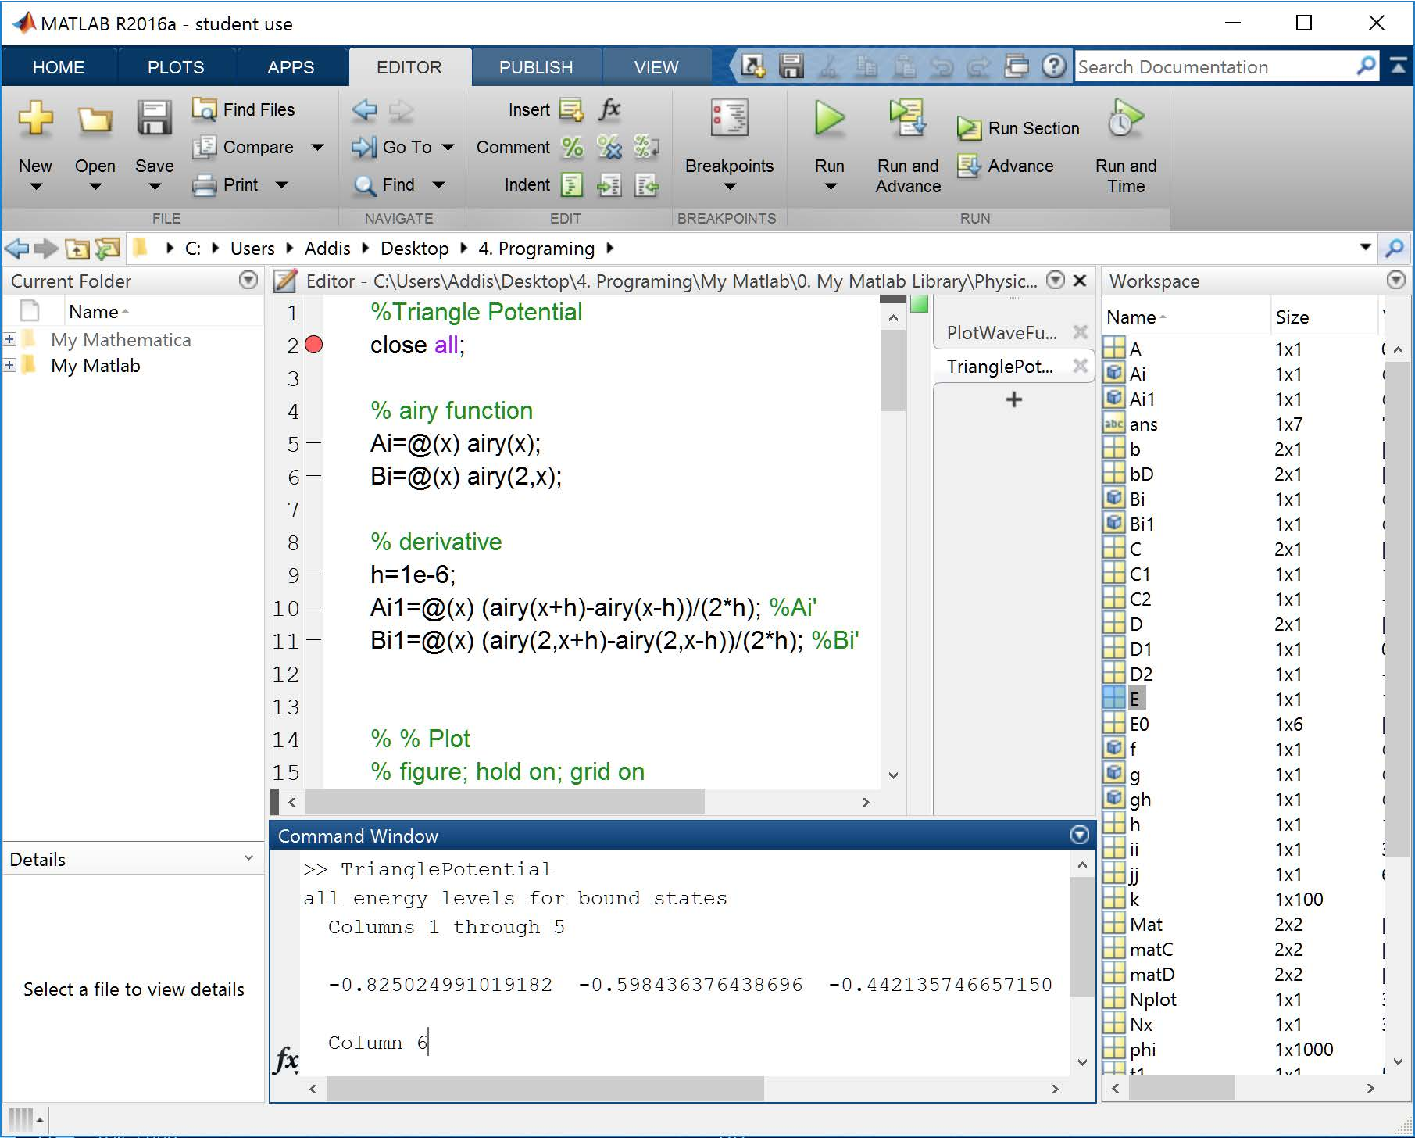
\includegraphics[width= 14cm]{./figures/Matlab1.pdf}
\caption{Matlab 的 IDE 界面}\label{Matlab_fig1}
\end{figure}

Matlab 的编程界面(\autoref{Matlab_fig1})属于\bb{集成开发环境(IDE/Integrated Develop Environment)},简而言之就是一切与 Matlab 编程有关的工作都可以在该界面完成\footnote{界面语言默认与操作系统语言相同,本书使用英文界面.}.以下介绍界面中常用的窗口.要选择显示的窗口,可在 Home 菜单中点击 Layout 按钮,并在 Show 下面勾选需要的窗口.

\bb{Editor} 用于编辑代码,同时具有自动检测语法错误,代码调试等功能.Matlab 的代码文件分为脚本文件和函数文件两种形式,后缀名都为 “.m”,用图1中 Editor 菜单栏的 Save 按钮可保存代码文件.Matlab 作为一种\bb{解释语言(Interpreted Language)}可以直接在 Editor 中运行源代码,无需传统的编译过程.为了让 Matlab 能运行代码文件,需要把文件所在的目录\footnote{在英文界面下 Matlab 不能识别中文目录,建议用英文命名文件夹.}添加到 Matlab 的搜索路径下.

\begin{figure}[ht]
\centering
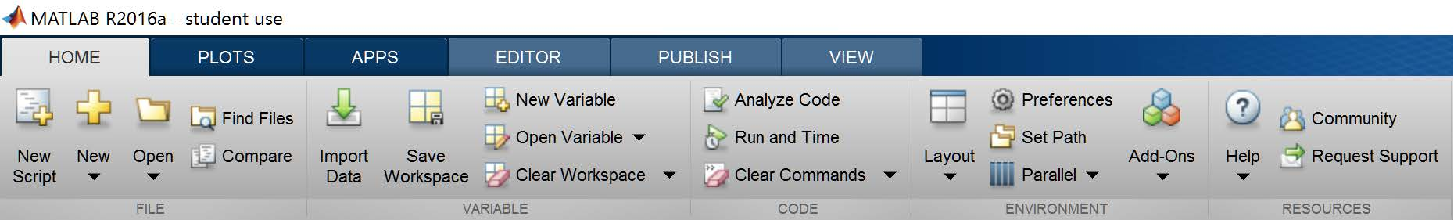
\includegraphics[width= 14cm]{./figures/Matlab2.pdf}
\caption{Home 菜单}\label{Matlab_fig2}
\end{figure}

如\autoref{Matlab_fig2},Home 菜单中的 Set Path 按钮可以设置 Matlab 的搜索路径.点开后用 Add Folder 按钮可以添加单个文件夹(不包含子文件夹),用 Add with Subfolders 添加文件夹(包含子文件夹).用 Remove 删除已添加的路径,用 Default 还原初始设置,用 Save 保存修改,用 Close 关闭窗口.若要运行程序,回到 Editor 菜单点击 Run 按钮即可.

\bb{Command Window} 主要用于输入临时指令或者调试程序,可输入除了函数定义外的任意指令.Command Window 只能按输入顺序执行,不方便修改和编辑,如果指令较长或有多个指令,应该使用 Editor.在 Command Window 中按回车执行输入的指令,按上箭头可重复已输入的指令.

\bb{Workspace} 用于查看 Matlab 当前的所有变量的列表.Matlab 的所有变量都可以理解为矩阵,单个值可理解为 \x{1×1} 的矩阵.列表中 Name 是变量名,Size 是矩阵维度,Value 是变量值,右上角的下拉菜单中的 Choose Columns 中还可设置显示更多属性,例如 Bytes 是占用字节数,Class 是变量类型,Min 是最小值,Max 是最大值,Mean 是平均值,Median 是中位数,Std 是标准差等.双击 Workspace 中的变量可显示变量值.

\subsection{Matlab Online}
Matlab Online 是 Matlab 网页版, 具有 Matlab 的基本功能,和类似于软件的界面,需要购买了正版 Matlab 的 Matlab 账号登录(学生账号也可以).若账号购买了工具箱(Toolbox),也可以使用对应的工具箱.本书官网 littleshi.cn/PhysWiki 提供免费的 Matlab 账号供读者试用和体验 Matlab Online.

\subsection{计算器}
下面我们仅用 Command Window 来熟悉 Matlab 的基本语法.我们先看如何把 Matlab 当做普通的科学计算器使用. 在 Command Window 中, “\x{>>}” 提示符表示用户在该位置输入命令, \x{ans} 是一个特殊的变量\upref{MatVar} 用于储存计算结果.
\begin{Command}
>> 1.2/3.4 + (5.6+7.8)*9 -1 \\
ans = 119.9529 \\
>> ans + 1\\
ans = 120.9529\\
>> 1/exp(1) \\
ans = 0.3679 \\
>> exp(-1i*pi)+1 \\
ans = 0
\end{Command}
常用的运算符号有
\begin{Command}
+,-,*,/,\^\ (指数)
\end{Command}
常用的数学函数有
\begin{Command}
sqrt(开方),exp,sin,cos,tan,cot,asin,acos,atan,acot,real(实部),imag(虚部),conj(共轭)
\end{Command}
等(三角函数前面加 \x{a} 代表其反函数).运算的优先顺序与数学上的习惯一样.注意这些函数的自变量都可以是复数.为了区分虚数单位 \x{i} 和变量 \x{i},好的习惯是在 \x{i} 前面加数字(上面的第三条命令). \x{pi} 是圆周率, 注意是小写.

\x{mod(N,n)} 是求余运算,计算 \x{N} 被 \x{n} 整除后的余数.注意这个函数有两个变量,用逗号隔开.要注意在 Matlab 中,这种有输入和输出的命令都是广义的\bb{函数(function)},不仅是数学函数.

\x{sign(num)} 函数用于求实数 \x{num} 的符号. 如果 \x{num > 0}, 则返回 1, 若 \x{num < 0} 则返回 $-1$, 若 \x{num = 0} 则返回 0.

用大写 \x{E} 或小写 \x{e} 表示科学计数法(不允许有空格),如 $2.997\times 10^8$ 表示为 \x{2.997e8} 或 \x{2.997e+8}.用小写 \x{pi} 表示圆周率,用 \x{exp(1)} 表示自然对数底,用 \x{1+2i} 或 \x{1+2j} 等表示复数,注意 \x{i} 和 \x{j} 前面不能有空格.

如果需要在输出中显示多位小数,可使用 \x{format long} 命令使结果显示为\bb{双精度}(约16位有效数字),用 \x{format short} 命令恢复默认格式.
\begin{Command}
>> format {\color{string}long}; pi \\
ans = 3.141592653589793 \\
>> exp(1) \\
ans = 2.718281828459046
\end{Command}